\documentclass{standalone}
\usepackage{tikz}
\usetikzlibrary{patterns, positioning}


\begin{document}
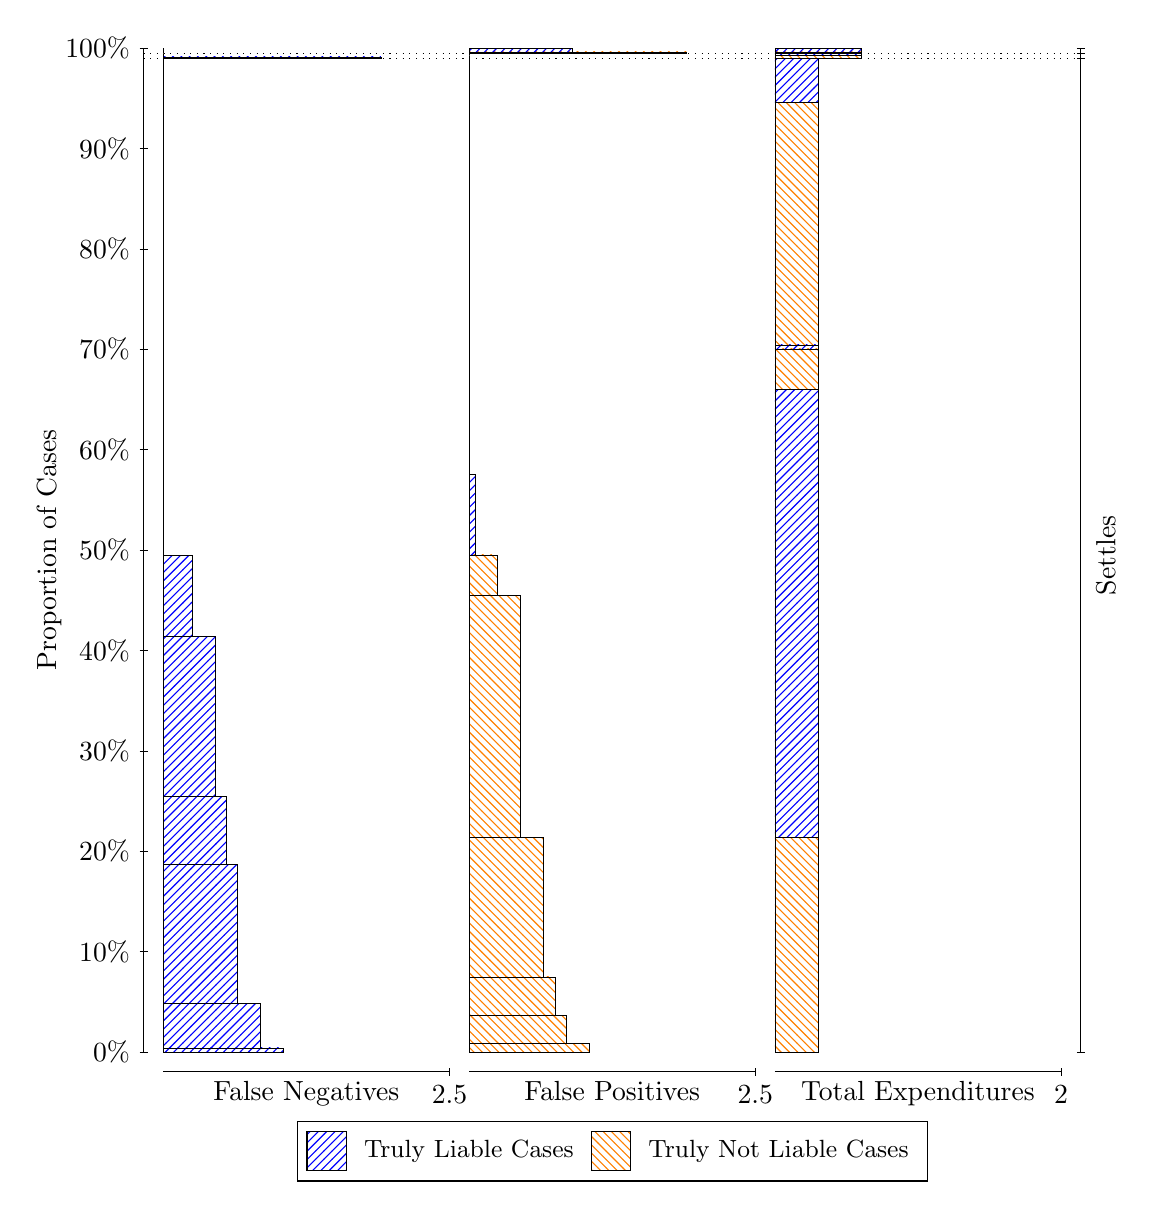
\begin{tikzpicture}
\draw[black, very thin] (1.5,1.75) -- (1.5,14.5);
\node[rotate=90, text=black, anchor=center] at (0.3, 8.125) {Proportion of Cases};
\draw[black, very thin] (1.45,1.75) -- (1.55,1.75);
\node[text=black, anchor=east] at (1.45, 1.75) {0\%};
\draw[black, very thin] (1.45,3.025) -- (1.55,3.025);
\node[text=black, anchor=east] at (1.45, 3.025) {10\%};
\draw[black, very thin] (1.45,4.3) -- (1.55,4.3);
\node[text=black, anchor=east] at (1.45, 4.3) {20\%};
\draw[black, very thin] (1.45,5.575) -- (1.55,5.575);
\node[text=black, anchor=east] at (1.45, 5.575) {30\%};
\draw[black, very thin] (1.45,6.85) -- (1.55,6.85);
\node[text=black, anchor=east] at (1.45, 6.85) {40\%};
\draw[black, very thin] (1.45,8.125) -- (1.55,8.125);
\node[text=black, anchor=east] at (1.45, 8.125) {50\%};
\draw[black, very thin] (1.45,9.4) -- (1.55,9.4);
\node[text=black, anchor=east] at (1.45, 9.4) {60\%};
\draw[black, very thin] (1.45,10.675) -- (1.55,10.675);
\node[text=black, anchor=east] at (1.45, 10.675) {70\%};
\draw[black, very thin] (1.45,11.95) -- (1.55,11.95);
\node[text=black, anchor=east] at (1.45, 11.95) {80\%};
\draw[black, very thin] (1.45,13.225) -- (1.55,13.225);
\node[text=black, anchor=east] at (1.45, 13.225) {90\%};
\draw[black, very thin] (1.45,14.5) -- (1.55,14.5);
\node[text=black, anchor=east] at (1.45, 14.5) {100\%};

\draw[black, very thin] (13.4,1.75) -- (13.4,14.5);
\draw[black, very thin] (13.35,1.75) -- (13.45,1.75);
\node[anchor=west] at (13.35, 1.75) {};
\draw[black, very thin] (13.35,14.366) -- (13.45,14.366);
\node[anchor=west] at (13.35, 14.366) {};
\draw[black, very thin] (13.35,14.429) -- (13.45,14.429);
\node[anchor=west] at (13.35, 14.429) {};
\draw[black, very thin] (13.35,14.5) -- (13.45,14.5);
\node[anchor=west] at (13.35, 14.5) {};

\draw[black, very thin, pattern color=blue, pattern=north east lines] (1.75,1.75) rectangle (3.276,1.803);
\draw[black, very thin, pattern color=blue, pattern=north east lines] (1.75,1.803) rectangle (2.9853,2.3626);
\draw[black, very thin, pattern color=blue, pattern=north east lines] (1.75,2.3626) rectangle (2.6947,4.1324);
\draw[black, very thin, pattern color=blue, pattern=north east lines] (1.75,4.1324) rectangle (2.5493,4.995);
\draw[black, very thin, pattern color=blue, pattern=north east lines] (1.75,4.995) rectangle (2.404,7.0287);
\draw[black, very thin, pattern color=blue, pattern=north east lines] (1.75,7.0287) rectangle (2.1133,8.0536);
\draw[black, very thin, pattern color=orange, pattern=north west lines] (1.75,8.0536) rectangle (1.75,14.366);
\draw[black, very thin, pattern color=blue, pattern=north east lines] (1.75,14.366) rectangle (4.5113,14.388);
\draw[black, very thin, pattern color=orange, pattern=north west lines] (1.75,14.388) rectangle (1.75,14.429);
\draw[black, very thin, pattern color=orange, pattern=north west lines] (1.75,14.429) rectangle (1.75,14.451);
\draw[black, very thin, pattern color=blue, pattern=north east lines] (1.75,14.451) rectangle (1.75,14.5);
\draw[black, very thin, pattern color=orange, pattern=north west lines] (5.6333,1.75) rectangle (7.1593,1.856);
\draw[black, very thin, pattern color=orange, pattern=north west lines] (5.6333,1.856) rectangle (6.8687,2.2152);
\draw[black, very thin, pattern color=orange, pattern=north west lines] (5.6333,2.2152) rectangle (6.7233,2.7045);
\draw[black, very thin, pattern color=orange, pattern=north west lines] (5.6333,2.7045) rectangle (6.578,4.4743);
\draw[black, very thin, pattern color=orange, pattern=north west lines] (5.6333,4.4743) rectangle (6.2873,7.5501);
\draw[black, very thin, pattern color=orange, pattern=north west lines] (5.6333,7.5501) rectangle (5.9967,8.0625);
\draw[black, very thin, pattern color=blue, pattern=north east lines] (5.6333,8.0625) rectangle (5.706,9.0875);
\draw[black, very thin, pattern color=blue, pattern=north east lines] (5.6333,9.0875) rectangle (5.6333,14.366);
\draw[black, very thin, pattern color=orange, pattern=north west lines] (5.6333,14.366) rectangle (5.6333,14.407);
\draw[black, very thin, pattern color=blue, pattern=north east lines] (5.6333,14.407) rectangle (5.6333,14.429);
\draw[black, very thin, pattern color=orange, pattern=north west lines] (5.6333,14.429) rectangle (8.3947,14.451);
\draw[black, very thin, pattern color=blue, pattern=north east lines] (5.6333,14.451) rectangle (6.9413,14.5);
\draw[black, very thin, pattern color=orange, pattern=north west lines] (9.5167,1.75) rectangle (10.062,4.4743);
\draw[black, very thin, pattern color=blue, pattern=north east lines] (9.5167,4.4743) rectangle (10.062,10.165);
\draw[black, very thin, pattern color=orange, pattern=north west lines] (9.5167,10.165) rectangle (10.062,10.678);
\draw[black, very thin, pattern color=blue, pattern=north east lines] (9.5167,10.678) rectangle (10.062,10.731);
\draw[black, very thin, pattern color=orange, pattern=north west lines] (9.5167,10.731) rectangle (10.062,13.807);
\draw[black, very thin, pattern color=blue, pattern=north east lines] (9.5167,13.807) rectangle (10.062,14.366);
\draw[black, very thin, pattern color=orange, pattern=north west lines] (9.5167,14.366) rectangle (10.607,14.407);
\draw[black, very thin, pattern color=blue, pattern=north east lines] (9.5167,14.407) rectangle (10.607,14.429);
\draw[black, very thin, pattern color=orange, pattern=north west lines] (9.5167,14.429) rectangle (10.607,14.451);
\draw[black, very thin, pattern color=blue, pattern=north east lines] (9.5167,14.451) rectangle (10.607,14.5);
\draw[black, dotted] (1.5,14.366) -- (13.4,14.366);
\draw[black, dotted] (1.5,14.429) -- (13.4,14.429);
\draw[black, very thin] (1.75,1.5) -- (5.3833,1.5);
\node[text=black, anchor=north] at (3.5667, 1.5) {False Negatives};
\draw[black, very thin] (5.3833,1.45) -- (5.3833,1.55);
\node[text=black, anchor=north] at (5.3833, 1.45) {2.5};

\draw[black, very thin] (5.6333,1.5) -- (9.2667,1.5);
\node[text=black, anchor=north] at (7.45, 1.5) {False Positives};
\draw[black, very thin] (9.2667,1.45) -- (9.2667,1.55);
\node[text=black, anchor=north] at (9.2667, 1.45) {2.5};

\draw[black, very thin] (9.5167,1.5) -- (13.15,1.5);
\node[text=black, anchor=north] at (11.333, 1.5) {Total Expenditures};
\draw[black, very thin] (13.15,1.45) -- (13.15,1.55);
\node[text=black, anchor=north] at (13.15, 1.45) {2};

\node[text=black, centered, rotate=90] at (13.72, 8.0581) {Settles};



\draw (7.449999999999999,1.5) node[draw=none] (baseCoordinate) {};
\begin{scope}[align=center]
        \matrix[scale=0.5, draw=black, below=0.5cm of baseCoordinate, nodes={draw}, column sep=0.1cm]{
            \node[rectangle, draw, minimum width=0.5cm, minimum height=0.5cm, pattern color=blue, pattern=north east lines] {}; &
            \node[draw=none, font=\small, text=black] (B) {Truly Liable Cases}; &
            \node[rectangle, draw, minimum width=0.5cm, minimum height=0.5cm, pattern color=orange, pattern=north west lines] {}; &
            \node[draw=none, font=\small, text=black] (B) {Truly Not Liable Cases}; \\
            };
\end{scope}

\end{tikzpicture}
\end{document}